
\documentclass[]{beamer}
% hyperref={pdfpagelabels=false} in [] bei documentclass

\usepackage[utf8]{inputenc}
\usepackage[T1]{fontenc}
\usepackage[english]{babel}
\usepackage{subfigure}
\usepackage{appendixnumberbeamer}
\usepackage{booktabs}
\usepackage{pgfplots}
\usepackage{xspace}
\usepackage{amsmath, amssymb, amsthm}
%\usepackage{footmisc}
\usepackage{csquotes}
\usepackage{tikz}
\usepackage[T1]{fontenc}

%usepackage[]{footmisc}
\definecolor{mycolor}{rgb}{0.92156,0.5058,0.105882}
\definecolor{mycolor2}{rgb}{.98039,.98039,.98039}
\usetheme[numbering=none, progressbar=frametitle]{metropolis}
%\metroset{numbering=none}

\title{The Hardness of ``Lemmings''}
\subtitle{Another NP-complete Game}

\author{Philip Geißler}
\date{May 14, 2018}

\usepackage{tikz}
%\usetikzlibrary{ipe, arrows.meta}
%\usepackage{mathtools}

\newcommand{\fn}[1]{{\footnote{\scriptsize{ #1 }}}}

\begin{document}

\frame{\titlepage}

%\section{introduction to the game}

\addcontentsline{toc}{section}{An Introduction to ``Lemmings''}
\begin{frame}{Lemmings - an Overview}
\begin{minipage}[t]{0.4\textwidth}
	\begin{figure}
		\includegraphics[width=\textwidth]{lemmings_cover.jpg}
		\caption{the game cover\footnotemark}
	\end{figure}
\end{minipage}
\begin{minipage}[t]{0.05\textwidth}
~
\end{minipage}
\begin{minipage}[t]{0.5\textwidth}
\vspace{0.5cm}
\begin{itemize}
\item released in 1991
\item published by Psygnosis
\item developed by DMA Design
\vspace{0.5cm}
\item single player
\item puzzle genre
\item real time strategy
\end{itemize}
\end{minipage}
\footnotetext{\scriptsize{\url{https://goo.gl/1fnsdu}} \cite{x1}}
\end{frame}


\begin{frame}{Lemmings - the Basics}
\begin{figure}
\includegraphics[height=0.7\textheight]{level1.png}
\caption{an exemplary level\fn{https://classicreload.com/lemmings.html}}
\end{figure}
\end{frame}
% hier dick labern über die einzelnen Funktionen und Optionen


%\addcontentsline{toc}{section}{Table of Contents}
\begin{frame}{Table of Contents}
%\setbeamertemplate{section in toc}[sections numbered]
\tableofcontents
\end{frame}

\section{Formalization}
\begin{frame}{Formalization}
\begin{itemize}
\item time and space is discrete in ``Lemmings''
\item all other parameters are also discrete
\item[$\rightarrow$] level and solution can be formalized
\end{itemize}
\begin{align*}
\texttt{level: } L &= (\text{limit\footnotemark}, \text{save}, \text{lems}, \text{start}, \text{wdt}, \text{hgt}, \text{grid}, \text{exit}, \text{skills})\\
\texttt{level size:~} |L| &\approx |grid| = constant \cdot wdt \cdot hgt\\
\texttt{solution: } S &= \{m_1, m_2, m_3, \cdots\}\\
\texttt{move:~} m_j &= (\text{time}, \text{x}, \text{y}, \text{\#lemming}, \text{\#skill})
\end{align*}
\footnotetext{\scriptsize{Assumption: bounded by polynomial time in the size of the level}}
\end{frame}

\begin{frame}{The Decision Problem}
%\center{}
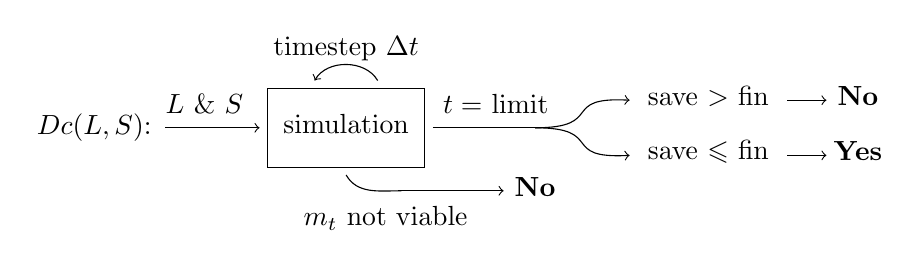
\begin{tikzpicture}
  \draw (-0.9,0) node {$Dc(L,S)$:};
  \draw[->] (-0,0) -- (1.2,0);
  \draw (0.5,0.3) node {$L$ \& $S$};
  \draw (1.3,.5) rectangle (3.3,-.5);
  \draw[<-] (2.3-0.4,0.6) to[out=60,in=120] (2.3+0.4,0.6);
  \draw (2.3,1.0) node {timestep $\Delta t$};
  \draw (2.3,.05) node {simulation};
  \draw (3.4,0) -- (3.4+1.3,0);
  \draw (4.2,0.3) node {$t = $ limit};
  \draw[->] (3.4+1.3,0) .. controls (4.3+1.3,0) and (3.7+1.3,0.4) .. (4.6+1.3,0.35);
  \draw[->] (3.4+1.3,0) .. controls (4.3+1.3,0) and (3.7+1.3,-0.4) .. (4.6+1.3,-0.35);
  \draw (4.6+1.3+1.0,0.4) node {save $>$ fin};
  \draw (4.6+1.3+1.0,-0.3) node {save $\leqslant$ fin};
  \draw[->] (4.6+1.3+1.0*2,0.35) -- (4.6+1.3+1.0*2+0.5,0.35);
  \draw[->] (4.6+1.3+1.0*2,-0.35) -- (4.6+1.3+1.0*2+0.5,-0.35);
  \draw (8.6+0.2,0.4) node {\textbf{No}};
  \draw (8.6+0.2,-0.3) node {\textbf{Yes}};
  \draw (2.3,-0.6) to[out=300,in=180] (2.3+0.7,-0.8);
  \draw[->] (2.3+0.7,-0.8) -- (2.3+2,-0.8);
  \draw (2.3+2+0.4,-0.75) node {\textbf{No}};
  \draw (2.8,-1.15) node {{$m_t$ not viable}};
\end{tikzpicture}\\
\vspace{0.7cm}
\begin{itemize}
\item $\forall \left( L \in \text{{LEMMINGS}} \right) ~\exists S_x \text{ with } Dc(L,S_x) = Yes$
\item[$\rightarrow$] LEMMINGS comprises all solvable levels
\item[$\hookrightarrow$] 1-LEMMINGS comprises all solvable levels with 1 Lemming
\item only LEMMINGS \& 1-LEMMINGS will be investigated further
\end{itemize}
\end{frame}

\subsection{3SAT tangent}
\begin{frame}{3 SAT}
\begin{align*}
\texttt{3SAT: } F &= \left(\overline{x_1} \vee x_2 \vee x_4\right) \wedge \left(\overline{x_3} \vee x_3 \vee \overline{x_4}\right) \wedge\left( \overline{x_1} \vee \overline{x_3}\right) \wedge \cdots\\
\texttt{exact 3SAT: } F &= \left(\overline{x_1} \vee x_2 \vee x_4\right) \wedge\left(\overline{x_4}\vee \overline{x_2} \vee x_3\right) \wedge \cdots
\end{align*}
\begin{itemize}
\vspace{-0.6cm}
\item 3SAT is NP-hard\fn{\url{https://dl.acm.org/citation.cfm?coll=GUIDE&dl=GUIDE&id=805047} \cite{x2}}\\
\vspace{-0.1cm}
\end{itemize}
\begin{align*}
\left(x_i \right) &\rightarrow \left(x_i \vee x_i \vee x_i \right) & \left(\right) &\rightarrow \left(x_i \vee x_i \vee x_i \right) \wedge \left(\overline{x_i} \vee \overline{x_i} \vee \overline{x_i} \right)\\
\left(x_i \vee x_j \right) &\rightarrow \left(x_i \vee x_j \vee x_i \right)
\end{align*}
\begin{itemize}
\vspace{-0.6cm}
\item[$\hookrightarrow$] exact 3SAT is also NP-hard
\vspace{-0.1cm}
\end{itemize}
\end{frame}

\section{Complexity Proofs}
\subsection{NP}
\begin{frame}{LEMMINGS $\in NP$}
\center{\Large{``[An input that returns `yes' must] be verifiable by deterministic computations that can be performed in polynomial time\fn{\url{https://goo.gl/5BZjRf} about problems in NP}''}}
\begin{itemize}
\item[$\rightarrow$] LEMMINGS be verified in polynomial time iff:
\item timesteps are evaluatable in time polynomial in the input size
\item moves are verifiable in time polynomial in the input size
\item timesteps are polynomial in the input size\fn{see assumptions}
\item moves are polynomial in the input size
\end{itemize}
\end{frame}

\begin{frame}{LEMMINGS $\in NP$}
\begin{figure}
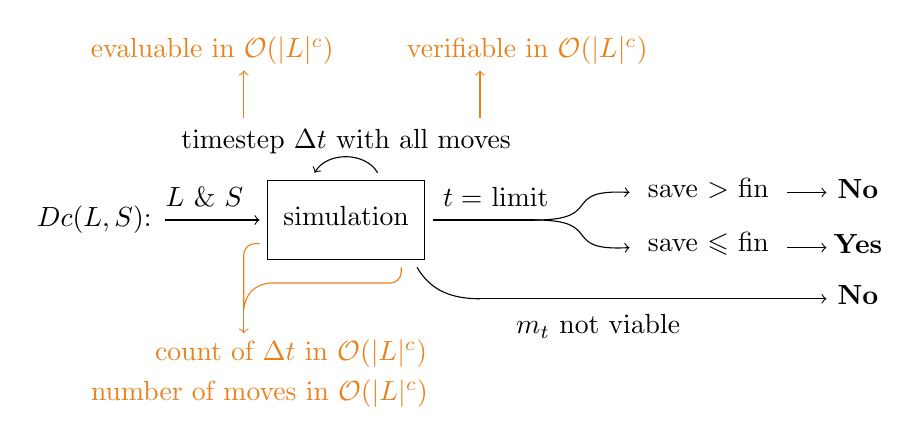
\begin{tikzpicture}
  \draw (-0.9,0) node {$Dc(L,S)$:};
  \draw[->] (-0,0) -- (1.2,0);
  \draw (0.5,0.3) node {$L$ \& $S$};
  \draw (1.3,.5) rectangle (3.3,-.5);
  \draw[<-] (2.3-0.4,0.6) to[out=60,in=120] (2.3+0.4,0.6);
  \draw (2.3,1.0) node {timestep $\Delta t$ with all moves};
  \draw (2.3,.05) node {simulation};
  \draw (3.4,0) -- (3.4+1.3,0);
  \draw (4.2,0.3) node {$t = $ limit};
  \draw[->] (3.4+1.3,0) .. controls (4.3+1.3,0) and (3.7+1.3,0.4) .. (4.6+1.3,0.35);
  \draw[->] (3.4+1.3,0) .. controls (4.3+1.3,0) and (3.7+1.3,-0.4) .. (4.6+1.3,-0.35);
  \draw (4.6+1.3+1.0,0.4) node {save $>$ fin};
  \draw (4.6+1.3+1.0,-0.3) node {save $\leqslant$ fin};
  \draw[->] (4.6+1.3+1.0*2,0.35) -- (4.6+1.3+1.0*2+0.5,0.35);
  \draw[->] (4.6+1.3+1.0*2,-0.35) -- (4.6+1.3+1.0*2+0.5,-0.35);
  \draw (8.6+0.2,0.4) node {\textbf{No}};
  \draw (8.6+0.2,-0.3) node {\textbf{Yes}};
  \draw (3.2,-0.6) to[out=300,in=180] (4,-1);
  \draw[->] (4,-1) -- (8.4,-1);
  \draw (8.8,-0.95) node {\textbf{No}};
  \draw (5.5,-1.35) node {{$m_t$ not viable}};
  
  %\visible<2>{
  \draw[mycolor, ->] (1,1.3) -- (1,1.9);
  \draw[mycolor, ->] (4,1.3) -- (4,1.9);
  
  \draw[mycolor, rounded corners=4pt]  (1.2,-0.3) -- (1,-0.3)  -- (1,-0.6) -- (1,-0.85) -- (1,-1.2) -- (1,-1) -- (1.2,-0.8) -- (3,-0.8) -- (3,-0.6);
  \draw[mycolor, ->] (1,-1) -- (1,-1.44);
  
  \draw[mycolor] (0.6,2.15) node {evaluable in $\mathcal{O}(|L|^c)$};
  \draw[mycolor] (4.6,2.15) node {verifiable in $\mathcal{O}(|L|^c)$};
  \draw[mycolor] (1.6,-1.7) node {count of $\Delta t$ in $\mathcal{O}(|L|^c)$};
  \draw[mycolor] (1.2,-2.2) node {number of moves in $\mathcal{O}(|L|^c)$};
  %}
\end{tikzpicture}
\caption{$S$ is verifiable for $L$ in $\mathcal{O}\left(|L|^{c'}\right)$}
\end{figure}
\end{frame}

\subsection{NP - Hard}
% 3SAT is NP-hard, so if we can reduce LEMMINGS to 3SAT, LEMMINGS is also NP-hard
\begin{frame}{LEMMINGS $\in NP \text{-} Hard$}
\center{\Large{goal: reduce LEMMINGS to 3SAT}}
\vspace{0.3cm}
\begin{itemize}
\item[$\rightarrow$] for each exact 3SAT problem, one can construct an equivalent problem in LEMMINGS
\begin{itemize}
\item clause conjunction $\rightarrow$ level $L_x$
\item literals \& clauses $\rightarrow$ gadgets
\item assignment of values to literals $\rightarrow$ strategy $S_{x}$ (1st part)
\item evaluation of the attempt for specific literals in each clause $\rightarrow$~strategy $S_{x}$ (2nd part)
\end{itemize}
\item for every satisfiable 3SAT, a strategy $S_x$ solving $L_x$ exists
\item for every solution of $L_x$, solution of 1 specific clause is found
\item[$\hookrightarrow$] if reduction is possible: $L_x \in$ LEMMINGS
\end{itemize}
\end{frame}

\begin{frame}{LEMMINGS $\in NP \text{-} Hard$}
\center{\Large{reduction example}}
\vspace{0.3cm}
\begin{align*}
\texttt{level:~~} &\left(\overline{x_1} \vee x_2 \vee x_4\right) \wedge\left(\overline{x_4}\vee \overline{x_2} \vee x_3\right) \wedge \left(\overline{x_3} \vee x_3 \vee \overline{x_4}\right)\\
\texttt{strategy pt.1:~~} &x_1 = false \hspace{1cm} x_2 = true\\ &x_3 = false \hspace{1cm} x_4 = false\\
\texttt{strategy pt.2:~~} &\left(\underline{\underline{\overline{x_1}}} \vee x_2 \vee x_4\right) \wedge\left(\underline{\underline{\overline{x_4}}}\vee \overline{x_2} \vee x_3\right) \wedge \left(\overline{x_3} \vee \underline{\underline{x_3}} \vee \overline{x_4}\right)\\
&\Rightarrow \overline{x_1} \wedge \overline{x_4} \wedge x_3
\\&= true \wedge true \wedge false
\\&= \underline{\underline{false}}
\end{align*}
\end{frame}

\begin{frame}{LEMMINGS $\in NP \text{-} Hard$}
\begin{figure}
\includegraphics[height=2.7cm]{g1.png}
\caption{the clause gadget \cite{p2}}
\end{figure}
\vspace{-0.5cm}
\begin{itemize}
\item the lemming can escape through digging a hole
\item each hole represents a check for the \textit{truthness} of the corresponding literal in the clause
\item[$\hookrightarrow$] if the literal is true, the entire clause evaluates to true
\end{itemize}
\end{frame}

\begin{frame}{LEMMINGS $\in NP \text{-} Hard$}
\begin{figure}
\includegraphics[height=2.7cm]{g2.png}
\caption{the variable gadget \cite{p2}}
\end{figure}
\vspace{-0.5cm}
\begin{itemize}
\item the lemming can escape through bashing and building a bridge
\item one side corresponds to $x_j = true$, the other to $x_j = false$
\item the clause lemming falls through the chosen hole and dies if he chose wrong
\item[$\hookrightarrow$] if all clause lemmings can choose right, the variables satisfy the clause
\end{itemize}
\end{frame}

\begin{frame}{LEMMINGS $\in NP \text{-} Hard$}
\vspace{0.3cm}
\center{\Large{algorithm example}}
\vspace{-0.7cm}
\center
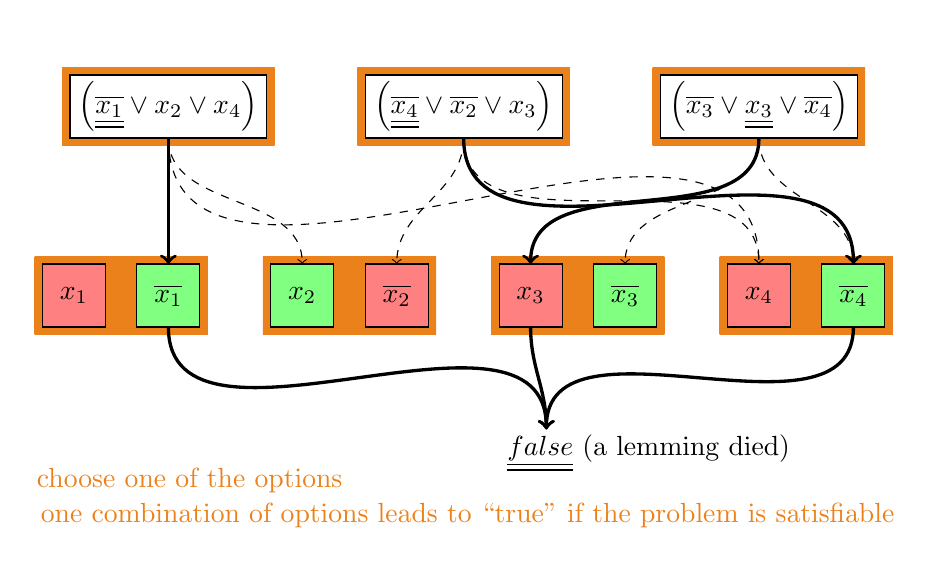
\begin{tikzpicture}
\shade[top color=mycolor, bottom color=mycolor] (-0.1+4.95-5,-0.1+2.0) rectangle (0.1+4.95-2.5,0.1+2.8);
\shade[top color=mycolor, bottom color=mycolor] (-0.1+4.95-1.25,-0.1+2.0) rectangle (0.1+4.95+1.25,0.1+2.8);
\shade[top color=mycolor, bottom color=mycolor] (-0.1+4.95+2.5,-0.1+2.0) rectangle (0.1+4.95+5,0.1+2.8);

\shade[top color=mycolor, bottom color=mycolor] (-.5,-.5) rectangle (1.7,.5);
\shade[top color=mycolor, bottom color=mycolor] (2.9+-.5,-.5) rectangle (2.9+1.7,.5);
\shade[top color=mycolor, bottom color=mycolor] (5.8+-.5,-.5) rectangle (5.8+1.7,.5);
\shade[top color=mycolor, bottom color=mycolor] (8.7+-.5,-.5) rectangle (8.7+1.7,.5);

\draw[text=mycolor] (1.47,-2.35) node {choose one of the options};

\draw (4.95-5,2.0)[fill=white] rectangle (4.95-2.5,2.8);
\draw (4.95-3.75,2.4) node {$\left(\underline{\underline{\overline{x_1}}} \vee x_2 \vee x_4\right)$};
\draw[very thick,->] (4.95-3.75,2.0) to[out=-90,in=90] (1*1.2,.4);
\draw[dashed,->] (4.95-3.75,2.0) to[out=-90,in=90] (1*0.5+2*1.2,.4);
\draw[dashed,->] (4.95-3.75,2.0) to[out=-90,in=90] (3*0.5+6*1.2,.4);
\draw (4.95-1.25,2.0)[fill=white] rectangle (4.95+1.25,2.8);
\draw (4.950,2.4) node {$\left( \underline{\underline{\overline{x_4}}}\vee \overline{x_2} \vee x_3\right)$};
\draw[very thick,->] (4.95,2.0) to[out=-90,in=90] (3*0.5+7*1.2,.4);
\draw[dashed,->] (4.95,2.0) to[out=-90,in=90] (1*0.5+3*1.2,.4);
\draw[dashed,->] (4.95,2.0) to[out=-90,in=90] (3*0.5+6*1.2,.4);
\draw (4.95+2.5,2.0)[fill=white] rectangle (4.95+5,2.8);
\draw (4.95+3.75,2.4) node {$\left(\overline{x_3} \vee \underline{\underline{x_3}} \vee \overline{x_4}\right)$};
\draw[very thick,->] (4.95+3.75,2.0) to[out=-90,in=90] (2*0.5+4*1.2,.4);
\draw[dashed,->] (4.95+3.75,2.0) to[out=-90,in=90] (2*0.5+5*1.2,.4);
\draw[dashed,->] (4.95+3.75,2.0) to[out=-90,in=90] (3*0.5+7*1.2,.4);

\draw (0*1.2-.4,.4)[fill=red!50!white] rectangle (0*1.2+.4,-.4);
\draw (0*1.2,0) node {$x_1$};
\draw (1*1.2-.4,.4)[fill=green!50!white] rectangle (1*1.2+.4,-.4);
\draw (1*1.2,0) node {$\overline{x_1}$};
\draw (1*0.5+2*1.2-.4,.4)[fill=green!50!white] rectangle (1*0.5+2*1.2+.4,-.4);
\draw (1*0.5+2*1.2,0) node {$x_2$};
\draw (1*0.5+3*1.2-.4,.4)[fill=red!50!white] rectangle (1*0.5+3*1.2+.4,-.4);
\draw (1*0.5+3*1.2,0) node {$\overline{x_2}$};
\draw (2*0.5+4*1.2-.4,.4)[fill=red!50!white] rectangle (2*0.5+4*1.2+.4,-.4);
\draw (2*0.5+4*1.2,0) node {$x_3$};
\draw (2*0.5+5*1.2-.4,.4)[fill=green!50!white] rectangle (2*0.5+5*1.2+.4,-.4);
\draw (2*0.5+5*1.2,0) node {$\overline{x_3}$};
\draw (3*0.5+6*1.2-.4,.4)[fill=red!50!white] rectangle (3*0.5+6*1.2+.4,-.4);
\draw (3*0.5+6*1.2,0) node {$x_4$};
\draw (3*0.5+7*1.2-.4,.4)[fill=green!50!white] rectangle (3*0.5+7*1.2+.4,-.4);
\draw (3*0.5+7*1.2,0) node {$\overline{x_4}$};

\draw[very thick,->] (2*0.5+4*1.2,-.4) to[out=-90,in=90] (6, -1.7);
\draw[very thick,->] (3*0.5+7*1.2,-.4) to[out=-90,in=90] (6, -1.7);
\draw[very thick,->] (1*1.2,-.4) to[out=-90,in=90] (6, -1.7);
\draw (7.3,-2) node {$\underline{\underline{false}}$ (a lemming died)};
\draw[text=mycolor] (5,-2.8) node {one combination of options leads to ``true'' if the problem is satisfiable};

\end{tikzpicture}
\end{frame}

\begin{frame}
\begin{figure}
\centering
\makebox[\columnwidth]{\includegraphics[width=1.15\textwidth]{g3.png}}
\end{figure}
\begin{align*}
\left(\overline{v_1} \vee v_2 \vee \overline{v_3}\right) \wedge \left(\overline{v_2} \vee v_3 \vee v_4\right) \wedge \left(v_1 \vee \overline{v_2} \vee \overline{v_4}\right) \wedge \left(\overline{v_1} \vee \overline{v_3} \vee \overline{v_4}\right) \text{  \cite{p2}}
\end{align*}
\end{frame}

\subsection{NP - Complete}
\begin{frame}{LEMMINGS $\in NP \text{-} Complete$}
\begin{figure}
\vspace{-0.33cm}
\includegraphics[width = 0.8\textwidth]{pnp2.png}
\caption{$NP \text{-} Complete$ as intersection of $NP$ and $NP$-$Hard$}
\end{figure}
\begin{itemize}
\item LEMMINGS $\in NP$ $\wedge$ LEMMINGS $\in NP \text{-} Hard$
\item[$\rightarrow$] LEMMINGS $\in NP \text{-} Complete$
\end{itemize}
\end{frame}

\section{Sources}
\begin{frame}{Quellen}
\begin{thebibliography}{9}
% DAS \FOOTNOTESIZE IMMER AN DEN ANFANG PACKEN
% bibitem([erstervornamebuschstabe][kapitelohnepunkte]-[footnotenumber])
\bibitem{p2}
Cormode, Graham, The Hardness of the Lemmings Game, or
Oh no, more NP-Completeness Proofs, 01.2004
\bibitem{x1}
Agent Palmer, Lemmings marched blindly into a Wonderful Gaming Legacy, 12.2014\\
\url{http://agentpalmer.com/10250/media/lemmings-marched-blindly-into-a-wonderful-gaming-legacy/}
\bibitem{x2}
Cook, Stephen A., The complexity of theorem-proving procedures, 05.1971\\
\url{https://dl.acm.org/citation.cfm?coll=GUIDE&dl=GUIDE&id=805047}
\end{thebibliography}
\end{frame}

\frame{\titlepage}
\frame{\titlepage}

\appendix


\begin{frame}{1-LEMMINGS $\in NP \text{-} Complete$}
\begin{itemize}
\item also in NP-Complete
\item much harder construction:
\end{itemize}
\begin{figure}
\includegraphics[width=0.8\textwidth]{g4.png}
\end{figure}
\end{frame}
\end{document}